%----------------------------------------------------------------------------------------
%	PACKAGES AND OTHER DOCUMENT CONFIGURATIONS
%----------------------------------------------------------------------------------------

\documentclass{article}

\usepackage{fancyhdr} % Required for custom headers
\usepackage{lastpage} % Required to determine the last page for the footer
\usepackage{extramarks} % Required for headers and footers
\usepackage[usenames,dvipsnames]{xcolor} % Required for custom colors
\usepackage{graphicx} % Required to insert images
\usepackage{listings} % Required for insertion of code
\usepackage{courier} % Required for the courier font
\usepackage{amsmath} % Used for matrices %
\usepackage{mathtools}
\usepackage{textcomp}
\usepackage{gensymb}
\usepackage{siunitx}
\usepackage{empheq}
\usepackage{ulem}
\usepackage{amssymb}

% Custom Commands %
\sisetup{output-exponent-marker=\ensuremath{\mathrm{E}}}
\definecolor{ao}{rgb}{0.0, 0.5, 0.0}

% Margins
\topmargin=-0.45in
\evensidemargin=0in
\oddsidemargin=0in
\textwidth=6.5in
\textheight=9.0in
\headsep=0.25in

\linespread{1.1} % Line spacing

% Set up the header and footer
\pagestyle{fancy}
\lhead{\hmwkAuthorName} % Top left header
\chead{\hmwkClass\ (\hmwkClassInstructor\ \hmwkClassTime): \hmwkTitle} % Top center head
\rhead{\firstxmark} % Top right header
\lfoot{\lastxmark} % Bottom left footer
\cfoot{} % Bottom center footer
\rfoot{Page\ \thepage\ of\ \protect\pageref{LastPage}} % Bottom right footer
\renewcommand\headrulewidth{0.4pt} % Size of the header rule
\renewcommand\footrulewidth{0.4pt} % Size of the footer rule

\setlength\parindent{0pt} % Removes all indentation from paragraphs

%----------------------------------------------------------------------------------------
%	CODE INCLUSION CONFIGURATION
%----------------------------------------------------------------------------------------

\definecolor{MyDarkGreen}{rgb}{0.0,0.4,0.0} % This is the color used for comments
\lstloadlanguages{Matlab} % Load Perl syntax for listings, for a list of other languages supported see: ftp://ftp.tex.ac.uk/tex-archive/macros/latex/contrib/listings/listings.pdf
\lstset{language=Matlab, % Use Perl in this example
        frame=single, % Single frame around code
        breakatwhitespace=true,
        breaklines = true,
        basicstyle=\small\ttfamily, % Use small true type font
        keywordstyle=[1]\color{Blue}\bf, % Perl functions bold and blue
        keywordstyle=[2]\color{Purple}, % Perl function arguments purple
        keywordstyle=[3]\color{Blue}\underbar, % Custom functions underlined and blue
        identifierstyle=, % Nothing special about identifiers                                         
        commentstyle=\usefont{T1}{pcr}{m}{sl}\color{MyDarkGreen}\small, % Comments small dark green courier font
        stringstyle=\color{Purple}, % Strings are purple
        showstringspaces=false, % Don't put marks in string spaces
        tabsize=5, % 5 spaces per tab
        %
        % Put standard Perl functions not included in the default language here
        morekeywords={rand},
        %
        % Put Perl function parameters here
        morekeywords=[2]{on, off, interp},
        %
        % Put user defined functions here
        morekeywords=[3]{test},
       	%
        morecomment=[l][\color{Blue}]{...}, % Line continuation (...) like blue comment
        numbers=left, % Line numbers on left
        firstnumber=1, % Line numbers start with line 1
        numberstyle=\tiny\color{Blue}, % Line numbers are blue and small
        stepnumber=1 % Line numbers go in steps of 1
        }

% Creates a new command to include a script, the first parameter is the filename of the script (without .pl), the second parameter is the caption
\newcommand{\script}[2]{
\begin{itemize}
\item[]\lstinputlisting[caption=#2,label=#1]{#1.m}
\end{itemize}
}

%----------------------------------------------------------------------------------------
%	DOCUMENT STRUCTURE COMMANDS
%	Skip this unless you know what you're doing
%----------------------------------------------------------------------------------------

% Header and footer for when a page split occurs within a problem environment
\newcommand{\enterProblemHeader}[1]{
\nobreak\extramarks{#1}{#1 continued on next page\ldots}\nobreak
\nobreak\extramarks{#1 (continued)}{#1 continued on next page\ldots}\nobreak
}

% Header and footer for when a page split occurs between problem environments
\newcommand{\exitProblemHeader}[1]{
\nobreak\extramarks{#1 (continued)}{#1 continued on next page\ldots}\nobreak
\nobreak\extramarks{#1}{}\nobreak
}

\setcounter{secnumdepth}{0} % Removes default section numbers
\newcounter{homeworkProblemCounter} % Creates a counter to keep track of the number of problems

\newcommand{\homeworkProblemName}{}
\newenvironment{homeworkProblem}[1][Problem \arabic{homeworkProblemCounter}]{ % Makes a new environment called homeworkProblem which takes 1 argument (custom name) but the default is "Problem #"
\stepcounter{homeworkProblemCounter} % Increase counter for number of problems
\renewcommand{\homeworkProblemName}{#1} % Assign \homeworkProblemName the name of the problem
\section{\homeworkProblemName} % Make a section in the document with the custom problem count
\enterProblemHeader{\homeworkProblemName} % Header and footer within the environment
}{
\exitProblemHeader{\homeworkProblemName} % Header and footer after the environment
}

\newcommand{\problemAnswer}[1]{ % Defines the problem answer command with the content as the only argument
\noindent\framebox[\columnwidth][c]{\begin{minipage}{0.98\columnwidth}#1\end{minipage}} % Makes the box around the problem answer and puts the content inside
}

\newcommand{\homeworkSectionName}{}
\newenvironment{homeworkSection}[1]{ % New environment for sections within homework problems, takes 1 argument - the name of the section
\renewcommand{\homeworkSectionName}{#1} % Assign \homeworkSectionName to the name of the section from the environment argument
\subsection{\homeworkSectionName} % Make a subsection with the custom name of the subsection
\enterProblemHeader{\homeworkProblemName\ [\homeworkSectionName]} % Header and footer within the environment
}{
\enterProblemHeader{\homeworkProblemName} % Header and footer after the environment
}

%----------------------------------------------------------------------------------------
%	NAME AND CLASS SECTION
%----------------------------------------------------------------------------------------

\newcommand{\hmwkTitle}{Assignment\ \#1} % Assignment title
\newcommand{\hmwkDueDate}{Thursday,\ October\ 1,\ 2015} % Due date
\newcommand{\hmwkClass}{CMSC\ 733} % Course/class
\newcommand{\hmwkClassTime}{11:00am} % Class/lecture time
\newcommand{\hmwkClassInstructor}{Aloimonos, Yiannis} % Teacher/lecturer
\newcommand{\hmwkAuthorName}{Kanishka Ganguly} % Your name

%----------------------------------------------------------------------------------------
%	TITLE PAGE
%----------------------------------------------------------------------------------------

\title{
\vspace{2in}
\textmd{\textbf{\hmwkClass:\ \hmwkTitle}}\\
\normalsize\vspace{0.1in}\small{Due\ on\ \hmwkDueDate}\\
\vspace{0.1in}\large{\textit{\hmwkClassInstructor\ \hmwkClassTime}}
\vspace{3in}
}

\author{\textbf{\hmwkAuthorName}}
\date{09/28/2015} % Insert date here if you want it to appear below your name

%----------------------------------------------------------------------------------------

\begin{document}

\maketitle

%----------------------------------------------------------------------------------------
%	TABLE OF CONTENTS
%----------------------------------------------------------------------------------------

%\setcounter{tocdepth}{1} % Uncomment this line if you don't want subsections listed in the ToC

\newpage
\tableofcontents
\newpage

%----------------------------------------------------------------------------------------
%	PROBLEM 1
%----------------------------------------------------------------------------------------

% To have just one problem per page, simply put a \clearpage after each problem

\begin{homeworkProblem}
\script{code/Q1}{Image Projection}

\begin{homeworkSection}{(a)} 
We know that the camera has \textbf{f = 1}, \textbf{origin at (0, 0, -3)} and is rotated at \textbf{-45 \degree}\\
In above code, lines \textit{13} to \textit{20} define the world coordinates of the cube and line \textit{26} takes into account the rotation of the camera at \textit{-45 \degree}.\\
Line \textit{29} takes care of the translation of the camera with origin at (0, 0, -3).\\
Also, we have the focal length of the camera as $f = 1$ which is used in Line \textit{33}.\\
This gives us the projection matrix:\\
\[
Pr = 
\begin{bmatrix}
0.5253 & 0 & -0.8509 & 2.5527 \\
0 & 1.0000 & 0 & 0 \\
0.8509 & 0 & 0.5253 & -1.5760
\end{bmatrix}
\]
\end{homeworkSection}

\begin{homeworkSection}{(b)} 
Using projection matrix \begin{verb} Pr \end{verb} we convert each of the coordinates in \begin{verb} world \end{verb} in Line \textit{23} to get the non-homogenous image coordinates as:
\begin{itemize}
\item $p_5 = (2.553, 0.500, -1.576)$
\item $p_6 = (3.078, 0.500, -0.725)$
\item $p_7 = (2.227, 0.500, -0.200)$
\item $p_8 = (1.702, 0.500, -1.051)$
\end{itemize}
Now, we divide the $x$, $y$ and $z$ coordinates by the $z$ coordinate to get the homogenous image coordinates as:
\begin{itemize}
\item ${p_5}_{homogenous} = (-1.620, -0.317, 1)$
\item ${p_6}_{homogenous} = (-4.245, -0.690, 1)$
\item ${p_7}_{homogenous} = (-11.150, -2.503, 1)$
\item ${p_8}_{homogenous} = (-1.620, -0.476, 1)$
\end{itemize}
\end{homeworkSection}

\begin{homeworkSection}{(c)} 
Geometrically, the first three columns of the projection matrix gives us the 3 vanishing points corresponding to the 3 parallel lines.\\
So, we have:\\
\[
Pr = 
\begin{bmatrix}
\textcolor{red}{0.5253} & \textcolor{ao}{0} & \textcolor{blue}{-0.8509} & 2.5527 \\
\textcolor{red}{0} & \textcolor{ao}{1.0000} & \textcolor{blue}{0} & 0 \\
\textcolor{red}{0.8509} & \textcolor{ao}{0} & \textcolor{blue}{0.5253} & -1.5760
\end{bmatrix}
\]
with the red, green and blue columns representing the $x$, $y$ and $z$ coordinates of the vanishing points of the 3 parallel lines respectively.\\
\end{homeworkSection}

\begin{homeworkSection}{(d)}
Let $p_5 = (2.553, 0.500, -1.576)$ and $p_7 = (2.227, 0.500, -0.200)$ be the camera coordinates of $P_5$ and $P_7$.\\
To compute the vanishing point of line $P5-P7$, we have the following equation for a line in 3-D:
\begin{align}
\frac{x-x_1}{x_2-x_1} = \frac{y-y_1}{y_2-y_1} = \frac{z-z_1}{z_2-z_1} = t
\end{align}
where $t$ is some parameter.\\

We take a vector $\vec{v}$ that is parallel to the line and we can write it as:
\begin{align}
\vec{v} = <0.283,0,-1.776>
\end{align}

In vector form, the line is:
\begin{align}
\vec{r} = <2.553, 0.5, -1.756> + <0.283,0,-1.776>t\\
\text{Or, we have}\nonumber \\
x = 2.553 + 0.283t\\
y = 0.5 + 0t\\
z = -1.756 -1.776t
\end{align}

We know, by definition, that the vanishing point of a line is the projection of that point at infinity. So, as parameter $t \to \infty$, we have the following homogenous coordinates:
\begin{align}
\frac{x}{z} \approx 0.283/1.776 = 0.1593\\
\frac{y}{z} \approx 0/1.776 = 0\\
\frac{z}{z} = 1
\end{align}

Thus, the homogenous coordinates of the vanishing point of line $P_5-P_7$ are (0.1237, 0, 1).
\end{homeworkSection}

\begin{homeworkSection}{(e)}
To obtain two ideal vanishing points, the optical axis of the camera should be in line with any of the principal axes of the world coordinate, namely the $X$, $Y$ or $Z$ axis.\\
Essentially, when the camera is placed such that the image plane is parallel to any one face of the cube (only a square is visible), then we can obtain two ideal vanishing points.
\end{homeworkSection}

\end{homeworkProblem}
\clearpage
%----------------------------------------------------------------------------------------
%	PROBLEM 2
%----------------------------------------------------------------------------------------

\begin{homeworkProblem}
Given that \begin{verb} P \end{verb} is a $3 \times 4$ camera projection matrix and \begin{verb} C \end{verb} is the camera center (in projective coordinates).\\
We know that
\begin{align}
P = [M | -MC]\\
\implies P = M[I | -C]\\
\text{So, multiplying by C on both sides,}\nonumber\\
P \times C = M[I | -C] \times C\\
\implies P \times C = M[0] = 0\\
\implies \underline{\underline{PC = 0}}
\end{align}

\end{homeworkProblem}

%----------------------------------------------------------------------------------------
%   PROBLEM 3
%----------------------------------------------------------------------------------------

\begin{homeworkProblem}

We know that \begin{verb} P \end{verb} is a $3 \times 4$ camera matrix and
\begin{align}
P = K \times R \times [I | -C]
\end{align}
Here, 
\begin{align}
K =
\begin{rcases}
\begin{bmatrix}
f & 0 & 0\\
0  & f & 0\\
0 & 0  & 1
\end{bmatrix}
\end{rcases}
\textbf{Calibration Matrix}
\\\nonumber
\\\nonumber
C =
\begin{rcases}
\begin{bmatrix}
C_x\\
C_y\\
C_z
\end{bmatrix}
\end{rcases}
\textbf{Camera Center}
\\\nonumber
\\\nonumber
R =
\begin{rcases}
\begin{bmatrix}
R_{11} & R_{12} & R_{13}\\
R_{21}  & R_{22} & R_{23}\\
R_{31} & R_{32}  & R_{33}
\end{bmatrix}
\end{rcases}
\textbf{Rotation Matrix}
\end{align}

Now, take the equation of the line joining the origin $\text{O} \equiv (0,0,0)$ and the camera center (world coordinate system) $\text{C} \equiv (C_x,C_y,C_z)$:\\
\begin{align}
x = C_x t\\
y = C_y t\\
z = C_z t
\end{align}

Let us consider any line parallel to this line joining $\text{OC}$.\\
On it, any general point has a coordinate as $X \equiv (C_xt + x', C_yt + y', C_zt + z') $\\
The image coordinate for above general point can be obtained using projection matrix \begin{verb} P \end{verb} as follows:
\begin{align}
X_{img} = PX\\
X_{img} = K \times R \times [I | -C] \times X\\
X_{img} = 
\begin{bmatrix}
f & 0 & 0\\
0 & f & 0\\
0 & 0 & 1
\end{bmatrix}
\times
\begin{bmatrix}
r_{11} & r_{12} & r_{13}\\
r_{21}  & r_{22} & r_{23}\\
r_{31} & r_{32}  & r_{33}
\end{bmatrix}
\times
\begin{bmatrix}
1 & 0 & 0 & -C_x\\
0 & 1 & 0 & -C_y\\
0 & 0 & 1 & -C_z
\end{bmatrix}
\times
\begin{bmatrix}
C_xt + x'\\
C_yt + y'\\
C_zt + z'
\end{bmatrix}
\end{align}
This gives us:
\[
\begin{bmatrix}
f(r_{11}(C_xt + x' - C_x)) + r_{12}(C_yt + y' - C_y) + r_{13}(C_zt + z' - C_z)\\
f(r_{21}(C_xt + x' - C_x)) + r_{22}(C_yt + y' - C_y) + r_{23}(C_zt + z' - C_z)\\
 (r_{31}(C_xt + x' - C_x)) + r_{32}(C_yt + y' - C_y) + r_{33}(C_zt + z' - C_z)
\end{bmatrix}
\]\\
As parameter $t \to \infty$, the vanishing point $V$ of the general point (in homogenous coordinates) becomes 
\begin{align}
V \equiv
\begin{bmatrix}
f(r_{11}C_x + r_{12}C_y + r_{13}C_z)\\
f(r_{21}C_x + r_{22}C_y + r_{23}C_z)\\
 (r_{31}C_x + r_{32}C_y + r_{33}C_z)
\end{bmatrix}\label{mat_23}
\end{align}
We know that the last $(4^{th})$ column of projection matrix is $P = -K \times R \times C$, or
\begin{align}
\begin{bmatrix}
-f(r_{11}C_x + r_{12}C_y + r_{13}C_z)\\
-f(r_{21}C_x + r_{22}C_y + r_{23}C_z)\\
-(r_{31}C_x + r_{32}C_y + r_{33}C_z)
\end{bmatrix}
\end{align}
which is equivalent to the matrix denoted by Eqn. \ref{mat_23} when taken in homogenous coordinate form.\\

Or, we can say that the $4^{th}$ column of the projection matrix denotes, geometrically, \uuline{the vanishing point of any line parallel to the line joining the camera center to the origin.}\\

Extending that logic to a line parallel to the $X$-axis $\equiv (C_xt + x', y', z')$, $Y$-axis $\equiv (x', C_yt + y', z')$ or the $Z$-axis $\equiv (x', y', C_zt + z')$, we get, in homogenous coordinates, the first 3 columns of the projection matrix \begin{verb} P \end{verb} respectively, which represent the vanishing points for the line.
\end{homeworkProblem}
\clearpage

%----------------------------------------------------------------------------------------
%   PROBLEM 4
%----------------------------------------------------------------------------------------

\begin{homeworkProblem}
\script{code/Q4}{Calibration}

We are given a $3 \times 4$ camera matrix as
\[
P = 
\begin{bmatrix}
\textcolor{blue}{\num{3.53e+2}} & \textcolor{blue}{\num{3.39e+2}} & \textcolor{blue}{\num{2.77e+2}} & \textcolor{red}{\num{1.44e+6}} \\
\textcolor{blue}{\num{-1.03e+2}} & \textcolor{blue}{\num{2.33e+1}} & \textcolor{blue}{\num{4.59e+2}} & \textcolor{red}{\num{-6.32e+5}} \\
\textcolor{blue}{\num{7.07e-1}} & \textcolor{blue}{\num{-3.53e-1}} & \textcolor{blue}{\num{6.12e-1}} & \textcolor{red}{\num{-9.18e+2}}
\end{bmatrix}
\]

We know that 
\begin{align}
P = [M | -MC] 
\end{align}
where $M$ is defined by the $3 \times 3$ matrix in blue and $-MC$ is defined by the $1 \times 3$ matrix in red.\\

Also, we know that 
\begin{align}
M = K \times R
\end{align}
where $K$ is the calibration matrix and $R$ is the rotation matrix.

Now, we perform RQ-Decomposition on matrix $M$ to get back the matrices $K$ and $R$.
RQ-Decomposition gives us two matrices $Q$ and $R$, one orthogonal and one upper-triangular in nature.\\
So, let $K = R_{QR}$ and let $R_{M} = Q$\\

Also, the matrix $-MC$ contains the camera center $C$ which we retrieve by solving:
\begin{align}
AX = B\\
\text{where AX = -MC and B = M}\nonumber\\
\implies C = -(-MC)/M
\end{align}

Now,
\[
K = 
\begin{bmatrix}
\alpha_x & s & x_0\\
0  & \alpha_y & y_0\\
0 & 0  & 1
\end{bmatrix}
\]
where $\alpha_x$ and $\alpha_y$ are the ``Focal Lengths'' in pixels, $x_0$ and $y_0$ are the coordinates of the image center in pixels and $s$ is the skew parameter.\\
So, comparing with the matrix $K$ obtained after RQ-Decomposition, we have:
\[
K = 
\begin{bmatrix}
\alpha_x & s & x_0\\
0  & \alpha_y & y_0\\
0 & 0  & 1
\end{bmatrix}
=
\begin{bmatrix}
-467.165 & -90.936 & -299.578\\
0  & -426.437 & -199.962\\
0 & 0  & 1
\end{bmatrix}
\]
Thus, we have the following:

\begin{align}
\textbf{Calibration Parameters}
\begin{cases}
\textbf{Focal Lengths}\quad (\alpha_x, \alpha_y)= (-467.165, -426.437)\\
\textbf{Image Centers}\quad (x_0, y_0)= (-299.578, -199.962)\\
\textbf{Skew Parameter}\quad s= -90.936\\
\end{cases}\\
\textbf{Camera Center}
\begin{cases}
(C_x, C_y, C_z)= (0.000232, 0.000191, 0.000044)
\end{cases}
\end{align}

\end{homeworkProblem}
\clearpage

%----------------------------------------------------------------------------------------
%   PROBLEM 5
%----------------------------------------------------------------------------------------
\begin{homeworkProblem}
It is given that three known points $\left\{A,B,C\right\}$ are collinear on a 3-D line and their images formed are $\left\{a, b,c\right\}$.\\
Assume $D$ to be the vanishing point of the 3-D line $ABC$ and its image is $d$.\\
Let us say that:
\begin{align}
A = (A_x, A_y, A_z)\\
B = (B_x, B_y, B_z)\\
C = (C_x, C_y, C_z)
\end{align}
are the coordinates of $A,B$ and $C$ respectively.\\

Now, let $f$ be the focal length of the camera and by convention, the optical axis lies along $Z$-axis.\\
So, we have:
\begin{align}
a = \Big( f\frac{A_x}{A_z},f\frac{A_y}{A_z},f \Big)\\
b = \Big( f\frac{B_x}{B_z},f\frac{B_y}{B_z},f \Big)\\
c = \Big( f\frac{C_x}{C_z},f\frac{C_y}{C_z},f \Big)
\end{align}

So, the line equation for the image points can be written as:
\begin{align}
x = f \frac{C_x}{C_z} + \Big( f \frac{C_x}{C_z} - \frac{B_x}{B_z} \Big) t\\
y = f \frac{C_y}{C_z} + \Big( f \frac{C_y}{C_z} - \frac{B_y}{B_z} \Big) t\\
\\
\implies t = \frac{cd}{bc}\\
\implies t = \frac{(u+1)q - (u+1)}{u + 1 - q}
\end{align}
where $u = \frac{ab}{bc}$ and $q = \frac{AC}{BC}$\\\\

Thus, vanishing point $d$ is:
\begin{align}
\Big( f \frac{C_x}{C_z} + \Big( f \frac{C_x}{C_z} - \frac{B_x}{B_z} \Big) t_1, f \frac{C_y}{C_z} + \Big( f \frac{C_y}{C_z} - \frac{B_y}{B_z} \Big) t_1, f \Big)
\end{align}
\end{homeworkProblem}
\clearpage
%----------------------------------------------------------------------------------------
%   PROBLEM 6
%----------------------------------------------------------------------------------------
\begin{homeworkProblem}
\begin{homeworkSection}{(a)} 
We have two sets of four known coplanar points, namely $\left\{A,B,C,D\right\}$ and $\left\{E,F,G,H\right\}$ and origin $O$.\\
Considering first set of points $\left\{O, A,B,C,D\right\}$, we have 4 lines $OA, OB, OC \enspace \text{and} \enspace OD$ passing through $O$. The cross-ratio for the angles represented by above lines can be given as:
\begin{align}
CR_O(A,B,C,D) = \frac{sin(OA, OC) sin(OB,OD)}{sin(OA, OD) sin(OB,OC)}
\end{align}
In a projective transformation, the cross-ratio remains invariant.\\
So, assuming that the point $M$ in the scene is projected to a point $M'$ coplanar to the points $A,B,C,D$, then we can find $M'$ using the cross-ratio as:
\begin{align}
CR_O(b,c,d,m) = CR_A(B,C,D,M')\\
CR_O(a,c,d,m) = CR_B(A,C,D,M')\\
CR_O(a,b,d,m) = CR_C(A,B,D,M')
\end{align}
Now, from the problem, since it is given that we know $A,B,C,D$ and $a,b,c,d$, we can calculate the coordinates of $M'$.\\\\
Similarly, assuming that point $M$ is projected to a point $M''$ coplanar to the points $E,F,G,H$, then we find $M''$ using cross-ratio as:
\begin{align}
CR_O(f,g,h,m) = CR_E(F,G,H,M'')\\
CR_O(e,g,h,m) = CR_F(E,G,H,M'')\\
CR_O(e,f,h,m) = CR_G(E,F,H,M'')
\end{align}
Thus, the viewing ray $Om$ can be \uuline{determined by the points $M'$ and $M''$}.
\end{homeworkSection}
\begin{homeworkSection}{(b)}
Consider the projection $A'$ of point $A$ on the plane $E,F,G,H$. We can obtain the point A' as:
\begin{align}
CR_e(f,g,h,a) = CR_E(F,G,H,A')\\
CR_f(e,g,h,a) = CR_F(E,G,H,A')\\
CR_g(e,f,h,a) = CR_G(E,F,H,A')
\end{align}

From Subsection 6(a), we have $M'$ and $M''$ and also we now have $A$ and $A'$. This gives us two rays $A A'$ and $M' M''$ from the camera center.\\
Thus \uuline{the intersection of $M' M''$ and $A A'$ gives us the camera center $O$}.
\end{homeworkSection}
\end{homeworkProblem}
\clearpage

%----------------------------------------------------------------------------------------
%   PROBLEM 7
%----------------------------------------------------------------------------------------
\begin{homeworkProblem}
\script{code/Q7}{Robot Vehicle}


\problemAnswer{ % Answer
\begin{center}
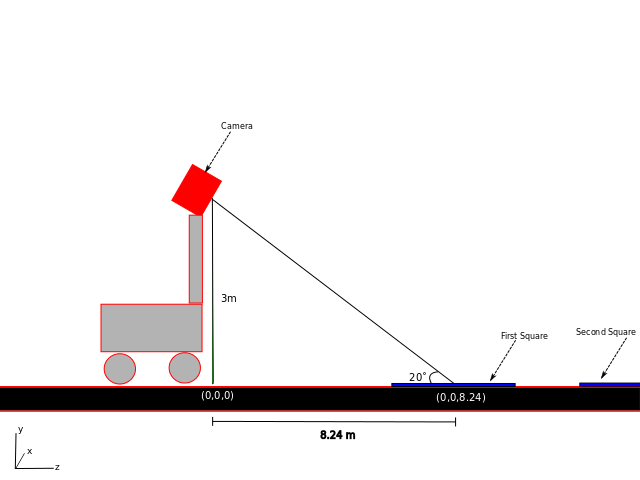
\includegraphics[width=0.75\columnwidth]{img/7_1.png} % Q7_1st Image
\end{center}
}
\vspace{20pt}
The basic setup.

\problemAnswer{ % Answer
\begin{center}
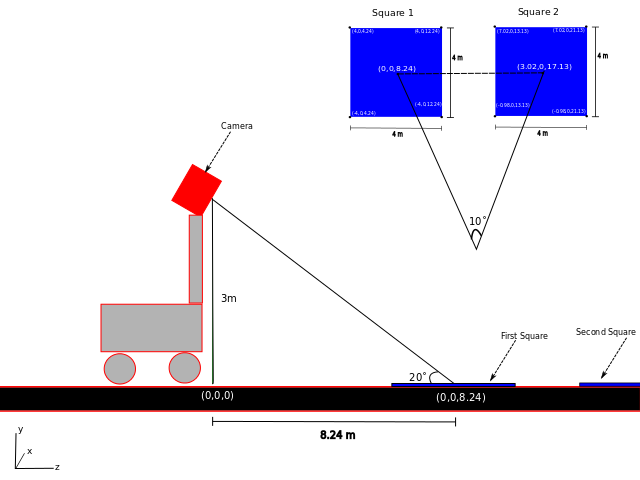
\includegraphics[width=0.75\columnwidth]{img/7_2.png} % Q7_2nd Image
\end{center}
}
\vspace{20pt}
The dimensions of the squares.

\problemAnswer{ % Answer
\begin{center}
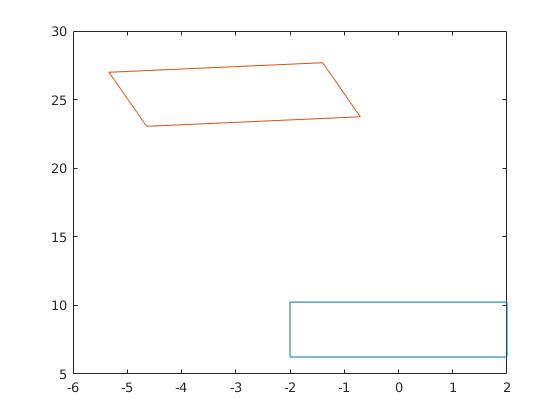
\includegraphics[width=0.75\columnwidth]{img/original.jpg} % Q7_1st Image
\end{center}
}
\vspace{20pt}
The original squares.

\problemAnswer{ % Answer
\begin{center}
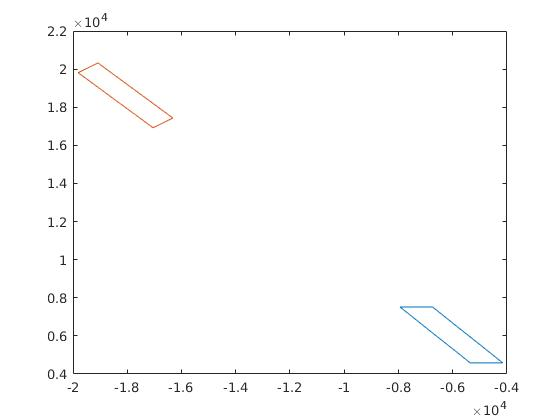
\includegraphics[width=0.75\columnwidth]{img/reconstructed.jpg} % Q7_2nd Image
\end{center}
}
\vspace{20pt}
The reconstructed squares.
\end{homeworkProblem}
\clearpage

%----------------------------------------------------------------------------------------
%   PROBLEM 8
%----------------------------------------------------------------------------------------
\begin{homeworkProblem}

\problemAnswer{ % Answer
\begin{center}
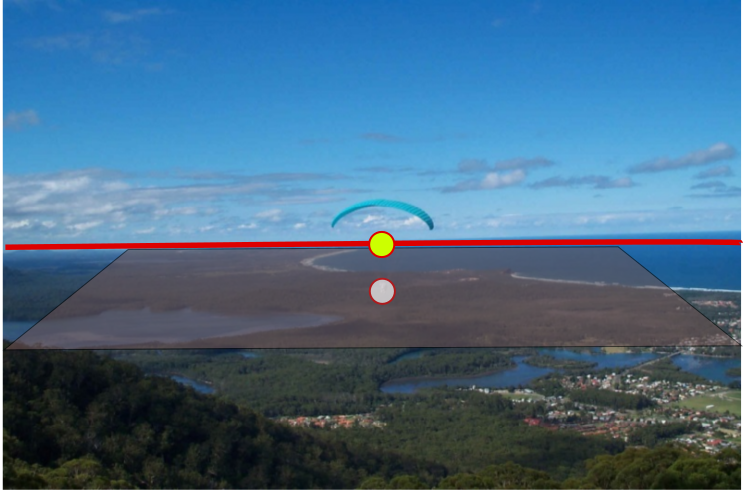
\includegraphics[width=0.75\columnwidth]{img/Q8.png} % Q8 Image
\end{center}
}
\vspace{20pt}

As can be seen from the modified figure, the brown plane shows the plane of the optical axis, which meets at the horizon to give the vanishing point in green.\\
All lines on this plane converge at the vanishing point.\\
The white circle represents the parachuter, who is lower than the vanishing point.\\
Thus, \uuline{the parachuter is lower than the person taking the picture}
\end{homeworkProblem}
\clearpage
%----------------------------------------------------------------------------------------

\end{document}